\documentclass{article}

\usepackage{biblatex}
\addbibresource{resources.bib}

\usepackage{graphicx}
\usepackage{tikz}
\usetikzlibrary{arrows}
\usetikzlibrary{quantikz}

\usepackage{physics}
\usepackage{amsthm}

\title{2QANIM: 2QAN Compiler Improved}
\author{S. S. Kahani}

\newtheorem{defn}{Definition}
\newtheorem{thrm}{Theorem}
\newtheorem{prob}{Problem}
\def\F{\mathcal{F}}

\begin{document}
  \maketitle
  \begin{abstract}
    { \color{blue} TODO }
  \end{abstract}

  \section{Introduction}
  
  While we are far from a general-purpose quantum computer 
  \cite{langione2019}
  that speeds up solving a vast range of problems, early real-world application could still be happening anytime soon by focusing on specific problems. \cite{preskill2018}
  Therefore, the importance of specific-purpose compilation is undeniable.
  
  Moreover, it is guessed that the early applications of quantum computers will include but not be limited to discrete optimizations and physical simulations.
  \cite{?} % 2019 paper
  This means that studying the compilation of k-local Hamiltonians is a meaningful choice as they play a significant role in the optimizations (like in QAOA \cite{farhi2014} and VQE \cite{peruzzo2014}) and undoubtedly in the physical simulations as well. 
  \cite{?} % TODO cite some review paper

  We may count the famous Trotter-Suzuki decomposition (see \ref{defn:trotter-suzuki}) as the first effort in compilation of Hamiltonians.
  But other works does not necessarily rely on that like \cite{campbell2019}.
  % TODO related work
  { \color{blue} TODO related work }
  
  This work is based on the 2QAN compiler \cite{lao2021} which is a hardware-aware compiler for 2-local Hamiltonians. The main contribution of this work is to improve the compilation of 2QAN by taking errors into account and introducing a new compilation algorithm. 

  % TODO classical compilation
  { \color{blue} TODO classical compilers }

  Here we introduce a hardware-aware compiler, starts from a 2-local Hamiltonian, defined in Definition \ref{defn:2-local-hamiltonian}, allocates qubits and generates intermediate gates that are studied in Section \ref{sec:two-qubit-gates} and finally transpile them to a lower-level gate-set. This compiler aims to reduce error in a reasonable compile-time, Therefore a detailed description of the assumed error model is given in Section \ref{sec:error-model}.

  \begin{figure}[h]
    \centering
  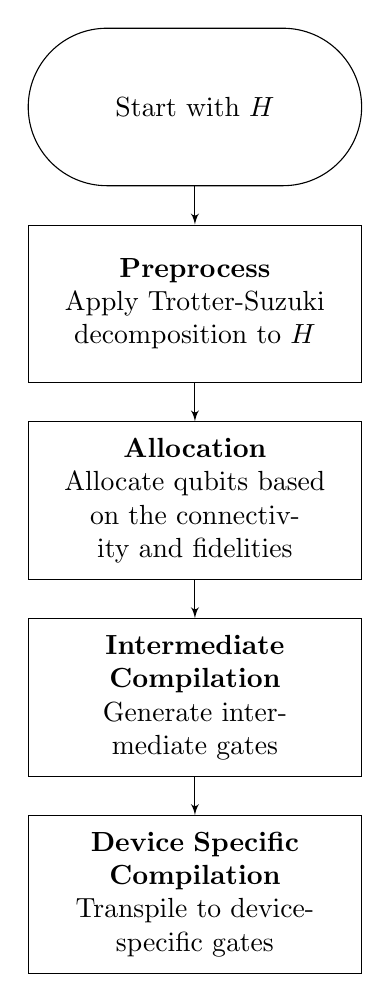
\begin{tikzpicture}[auto, node distance= 2.5cm,>=latex']
    \tikzstyle{block} = [draw, rectangle, text width=4cm, align=center, minimum height=2cm];
    \tikzstyle{rblock}=[block, rounded corners=1cm];
    \node [rblock] (a) {Start with $H$};
    \node [block, below of=a] (b) {\textbf{Preprocess} \\ Apply Trotter-Suzuki decomposition to $H$};
    \node [block, below of=b] (c) {\textbf{Allocation} \\
    Allocate qubits based on the connectivity and fidelities};
    \node [block, below of=c] (d) {\textbf{Intermediate Compilation} \\
    Generate intermediate gates};
    \node [block, below of=d] (e) {\textbf{Device Specific Compilation} \\
    Transpile to device-specific gates};
    \draw [->] (a) -- (b);
    \draw [->] (b) -- (c);
    \draw [->] (c) -- (d);
    \draw [->] (d) -- (e);
  \end{tikzpicture}
  \caption{The overview of the compilation process in 2QANIM}
\end{figure}

  \section{Basic Concepts}

  Because of the exponential growth of the number of gates in the compilation of a k-local term \cite{?}, setting $k=2$ is a reasonable choice for NISQ devices. This simplification not only helps us by reducing the number of gates, also enables us to use graph theory to define and analyze the problem, which is not easily possible for higher values of $k$.

  Here we introduce our notation for the Hamiltonian.

  \begin{defn}[2-local Hamiltonian]
    \label{defn:2-local-hamiltonian}
    Defining an $N$-qubit Hilbert space
    $\mathcal{H} := \otimes_{i=1}^{N} \mathcal{H_i}$, a 2-local Hamiltonian $H$ acting on it will be like
    \begin{equation}
      H := \sum_{i=1}^{k} h_i
    \end{equation}
    where each $h_i$ is a 2-local term, acting nontrivially on two specific qubits.
  \end{defn}
  \begin{defn}[Graph representation of a Hamiltonian]
    We will define the graph $G_H(V_H, E_H)$ to represent the Hamiltonian $H$, in a way that for each term $h_i$ in $H$, we have an edge $e_i$ between the two qubits it acts on.
  \end{defn}

  The very first step toward the compilation of a 2-local Hamiltonian is to apply the first-order Trotter-Suzuki decomposition \cite{trotter1959} to it. This decomposition is a way to approximate the time evolution of a Hamiltonian by a sequence of gates. 
  % TODO error of trotter

  \begin{defn}[Trotter-Suzuki decomposition]
    \label{defn:trotter-suzuki}
    The first order Trotter-Suzuki decomposition, decomposes a Hamiltonian $H$, into a set of two-qubit gates $g_i$s which associated with an edge like $e_i$.
    \begin{equation}
      \text{Target Gates} := \{ (g_i, e_i) \}
    \end{equation}
  \end{defn}

  The key feature of this decomposition (only the first order) is that the resulting gates can be applied in any order. This arbitrariness is not hold for a general quantum circuit and it may cause an advantage for a problem-specific compiler. % TODO bad wording
  
  % TODO what about higher order Trotter-Suzuki decomposition?
  % TODO see the new paper "Trotter Errors and the Emergence of Chaos in Quantum Simulation"

  \section{Intermediate Gate Set}

  In order to breakdown the process of compilation, which is surely a complex task, we use an intermediate description of the circuit, in terms of the intermediate gate set.

  This gate set is presumed to not be directly available on any device, but rather, it is easy to generate them relatively efficient on a quantum device. It is not wondering that we assume that the intermediate circuit must obey the topology of the device.

  While the implementation of one-qubit gates is not challenging, it is convenient to have all of the one-qubit gates, in the set, but for two qubit gates, many restrictions must be applied.

  The most important two-qubit gate that is often a part of any gate set is the CNOT gate. And because of the topology of the device, the CNOT might not be available on all pairs of qubits. Therefore we often add SWAP gate to make it possible all the way through the circuit, but optimality of the circuit is questionable in this case. Here we introduce a new gate, which is a generalization of the CNOT gate, which is shown to be more efficient than applying a SWAP gate.

  \subsection{Introducing Bridge Gates}
  For a simple case, that we have three qubits, called $a, b, c$, and we want to apply a CNOT gate on $(a, c)$, but the connectivity only allows us to apply a CNOT gate on $(a, b)$ and $(b, c)$, the first solution would be to use a SWAP gate, which is shown in figure \ref{fig:bridge-one-with-swap} (7 gates, depth of 7)
  While another approach is to use a bridge gate, which is shown in figure \ref{fig:bridge-one-with-bridge} (4 gates, depth of 4).

  \def\qceq{\midstick[3,brackets=none]{=}}
  \begin{figure}[h]
    \label{fig:bridge-one-with-swap}
    \centering
    \begin{quantikz}
    \lstick{a} & \ctrl{2} & \qw \qceq & \swap{1} & \qw & \swap{1} & \qw\qceq & \ctrl{1} & \targ{} & \ctrl{1} & \qw &\ctrl{1} & \targ{} & \ctrl{1} & \qw \\
    \lstick{b} & \qw & \qw & \swap{} & \ctrl{1} & \swap{} & \qw & \targ{} & \ctrl{-1}& \targ{} & \ctrl{1} & \targ{} & \ctrl{-1}& \targ{} & \qw \\
    \lstick{c} & \targ{} & \qw  & \qw & \targ{} & \qw & \qw & \qw & \qw & \qw & \targ & \qw & \qw & \qw & \qw  & \qw \\
    \end{quantikz}
    \caption{Applying a CNOT gate on $(a, c)$ using a SWAP gate}
  \end{figure}

  \begin{figure}[h]
    \label{fig:bridge-one-with-bridge}
    \centering
    \begin{quantikz}
    \lstick{a} & \ctrl{2} & \qw \qceq & \qw & \ctrl{1} & \qw & \ctrl{1} & \qw \\
    \lstick{b} & \qw & \qw & \ctrl{1} & \targ{} & \ctrl{1}  & \targ{} & \qw \\
    \lstick{c} & \targ{} & \qw & \targ{} & \qw  & \targ & \qw  & \qw &  \qw \\
    \end{quantikz}
    \caption{Applying a CNOT gate on $(a, c)$ using a bridge gate}
  \end{figure}
  
  This example, could be generalized and the bridge gate must be generalized as well. Hereby we define the generalized version of the bridge gate and we show the optimality of the bridge gate in terms of the number of CNOT gates and the depth of the circuit.

  \def\qceq{\midstick[6,brackets=none]{=}}
  \begin{defn}{Generalized Bridge Gate}
    For an even $n$
    \begin{align*} \mathrm{Bridge}(1, n) = &\prod_{i=1}^{n/2 - 1}\mathrm{CNOT}(i + 1, i)\mathrm{CNOT}(n - i + 1, n - i) \\ & \prod_{i=1}^{n/2 - 1}\mathrm{CNOT}(i, i + 1)\mathrm{CNOT}(n - i, n - i + 1) \\ & \mathrm{Bridge}(n/2 - 1, n/2)  \\
    & \qty(\prod_{i=1}^{n/2 - 1}\mathrm{CNOT}(i + 1, i)\mathrm{CNOT}(n - i + 1, n - i))^\dagger \\ 
    & \qty(\prod_{i=1}^{n/2 - 1}\mathrm{CNOT}(i, i + 1)\mathrm{CNOT}(n - i, n - i + 1))^\dagger
    \end{align*}
    but for an odd $n$, it is a little bit different.
  \end{defn}

  \begin{figure}[h]
    \centering
\begin{quantikz}
\qw &\ctrl{5}&\qw\qceq&\targ{}  & \qw     &\ctrl{1}& \qw    & \qw    & \qw    &\ctrl{1}& \qw     &\targ{}&\qw\\
\qw & \qw    & \qw    &\ctrl{-1}&\targ{}  & \targ{}&\ctrl{1}& \qw    &\ctrl{1}&\targ{} &\targ{}  &\ctrl{-1}&\qw\\
\qw & \qw    & \qw    & \qw     &\ctrl{-1}& \qw    & \targ{}&\ctrl{1}&\targ{} & \qw    &\ctrl{-1}&\qw & \qw \\
\qw & \qw    & \qw    & \qw     &\targ{}  & \qw    &\ctrl{1}& \targ{}&\ctrl{1}& \qw    &\targ{}  &\qw & \qw\\
\qw & \qw    & \qw    &\targ{}  &\ctrl{-1}&\ctrl{1}& \targ{}& \qw    &\targ{} &\ctrl{1}&\ctrl{-1}&\targ{}&\qw \\
\qw &\targ{} & \qw    &\ctrl{-1}& \qw     & \targ{}& \qw    & \qw    & \qw    &\targ{} & \qw     &\ctrl{-1}& \qw 
\end{quantikz}
    \caption{The bridge gate for $n=6$}
  \end{figure}

  \begin{thrm}
    Assume that we decomposed a CNOT between the first and the last qubits in a chain, in terms of local circuit.
    This circuit must carry information from the first bit to the last and reverse.
    For the forward information flow, the information is an $X$ gate placed on the first qubit, will travel along the circuit, so we need to have a consequential $n$ CNOT gates to carry this information. The same argument is valid for a backward series of gates.
    Ignoring the first and the last qubit, for each qubit this argument is also valid that, the gate in those series must not be the first neither the last CNOT gate applied on the qubit.
    Therefore, at least we need to have two series, each has to have a range of CNOT gates, before and after.
    One could easily manage to find out that the simplest structure would be similar (in terms of complexity) to the proposed bridge gate.
  \end{thrm}


  As far as we know, the family of bridge gates with more than one qubit in the chain is not studied yet, and neither implemented in any quantum compiler. 
  It can be easily shown that for a simple case like the one in the figure \ref{fig:bridge-simplification} that we need to swap and return the qubits, using bridge gate can reduce both depth and number of gates. 

  \begin{figure}
    a) \\
    \begin{center}
    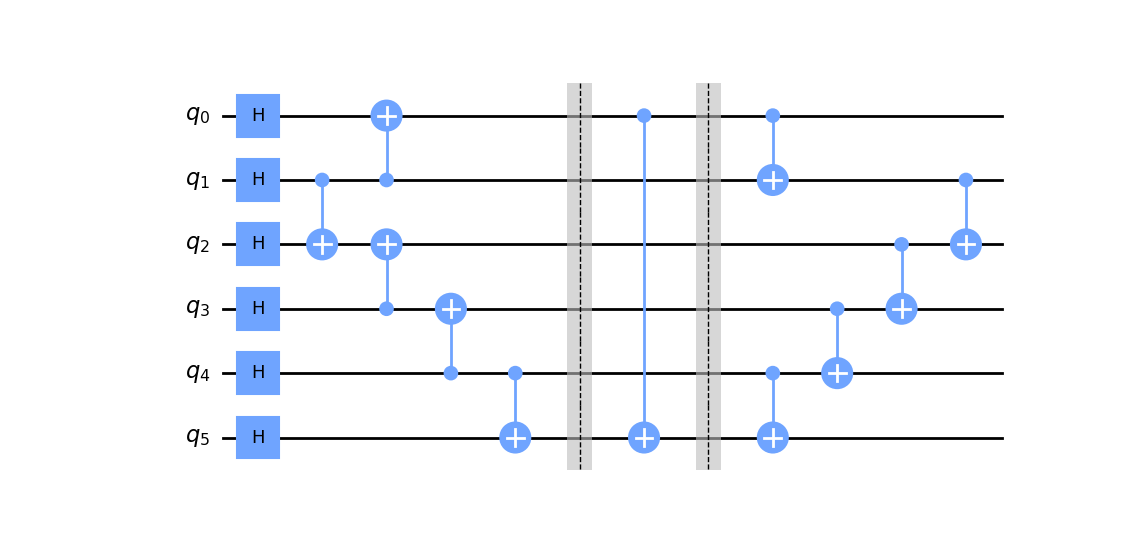
\includegraphics[width=0.9\textwidth]{../code/expm_1_bridge/out/original_circuit}
    \end{center}
    b) \\
    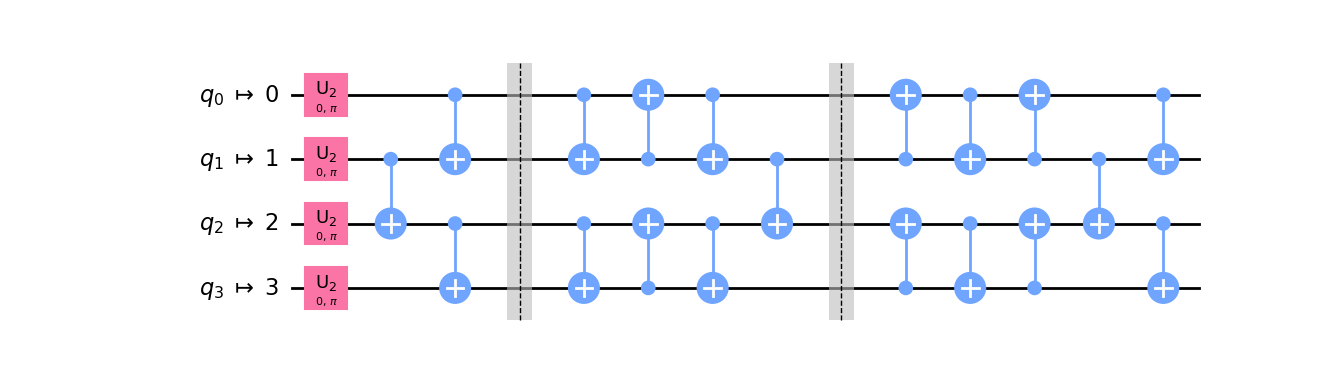
\includegraphics[width=0.9\textwidth]{../code/expm_1_bridge/out/transpiled_circuit_swap} \\
    c) \\
    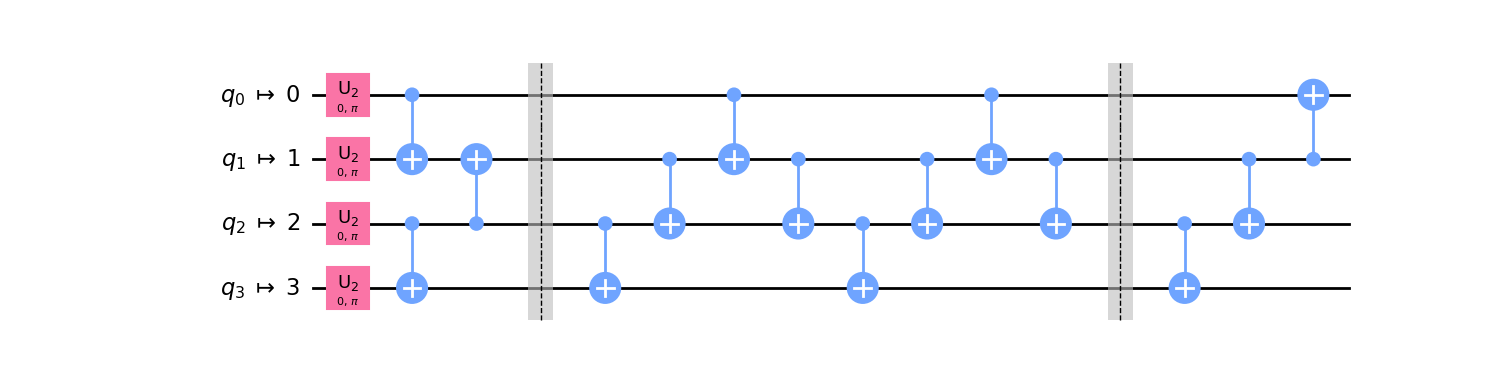
\includegraphics[width=0.9\textwidth]{../code/expm_1_bridge/out/transpiled_circuit_bridge}
    \caption{a) The original circuit, consisting of some local operations, then a far away CNOT and then some local operations. b) The circuit after transpiling using Qiskit. c) The circuit after transpiling using bridge gate as an intermediate gate.}
  \end{figure}
  \subsection{Unifying Gates}

  { \color{blue} TODO }
  We can combine two-qubit gates...

  \section{Error Model}
  \label{sec:error-model}
  Here we introduce a model to estimate errors of a circuit on a device.
  In this model, we take the average infidelity of a circuit as a measure of the error. In order to calculate the average (in)fidelity, we consider two different source of errors.

  \begin{itemize}
    \item \textbf{Decoherence}: When a qubit is left alone for some amount of time, it will decay to a random state. The average fidelity of the qubit can be written as:
    \begin{equation}
      \label{eq:decoherence}
      F_\text{decoherence}(t) = \exp(-\frac{t}{\tau_\text{decoherence}})
    \end{equation}
    \item \textbf{Gate Errors}: Any gate, specially the two-qubit gates, are not perfect. We can assign an average fidelity to each gate.
  \end{itemize}

  As for any parallel or sequential processes, the average fidelity of the circuit is the product of the average fidelity of each process, we use $-\log \F$, as a positive measure of error with additivity.

  Therefore, a device is defined as a tuple of the following:
  
  \begin{defn}[Device]
    \[ \text{Device} := (w_0 , G_d(V_d, E_d, w_\F)) \]
    where
    \[ \begin{cases}
    w_0 = \tau_\text{2-qubit gate time} / \tau_\text{decoherence}   \\ 
    w_\F(e) = -\log(\bar\F_\text{2-qubit gate on edge $e$} ) 
    \end{cases} \]
  \end{defn}
  
  \section{Problem Formulation}

  \subsection{NP-Hardness}
  Anyhow we define the problem, it is inevitable to have a subproblem like below

  \begin{prob}[Qubit Allocation]
    Given a graph that represents a Hamiltonian $G_H(V_H, E_H)$, find an allocation $\phi : V_H \to  V_d$ such the maximum number of edges in $E_H$ are mapped to $E_d$.
  \end{prob}

  We may use any other more complex criteria, such as minimizing estimated circuit error or minimizing the number of gates in the implemented circuits. But even in the simplest case, the problem is NP-hard, as the graph isomorphism problem can be reduced to it \cite{?}.

  But yet, this argument could be easily misinterepted into the fact that it is impossible to address the exact compilation algorithm in any case. It states that for an abitrary device graph, the problem is NP-hard. If we just add a simple constraint that the device graph has a bounded degree, then the problem is solvable in polynomial time. \cite{?}
  % TODO
  % TODO what about linear/lattice graph?

  \subsection{General Treatment}
  % TODO
  
  \section{Algorithms}
  \subsection{2QAN}
  \subsection{A*}
  % branching, consistency, admissibility
  \subsection{Resource Allocation}
  
\printbibliography

\end{document}